%!TEX root = ../PatilM-[RnD-MT]Report.tex

\chapter{Approach}
The conclusions drawn in the previous chapter, allow us the liberty of focusing specifically on the two most promising qualitative calculi $QTC_B$ and $ARGD$, for the purpose of developing an algorithm that centers around the utilization of either one or both of them, for the purpose of qualitatively representing physical space in our application of mobile robot navigation. Since the developed approach utilizes the QSRLib to implement the $QTC_B$ and $ARGD$ calculi further details on it will be provided in this chapter furthermore as the approach can be broken down into several subtasks this chapter is structured in the same manner as these subtasks.

%We use a minimum of two markers at every point on the opposing walls as this provides a sort of validation measure to ensure that the relations between the individual objects aren't unlikely, since each objects relation with the robot is a compliment of the other objects relation with respect to the robot. For example robot can't be moving to the left of both these objects if they lie on the opposite walls

%For the sake of simplifying our task we use aruco markers placed at various positions on the walls of the corridor, the use of aruco markers stems from the need to provide the QSRLib with cartesian coordinates of features or spatial entities with which the robot needs a relation. Additionally this allows us to simplfy the subtask of perception as we no longer need to detect robust features from the environment and can focus instead on the primary task of creating the qualitative abstractions and using them effectively.

\section{Approach}

\begin{figure}[h!]
	\centering
	\includegraphics[scale = 0.5]{"images/block diag"}
	\caption{Block diagram showing the input and output for each module along with the flow of control throughout the algorithm.}
	\label{fig:block-diag}
\end{figure}

\paragraph{Overview}The developed approach is a python implementation in the ROS ecosystem and can be broken down into three sub tasks or modules namely the qualitative perception module, the qualitative relation module and the qualitative control module. Each of these three modules deals with a crucial aspect of navigating using qualitative spatial representations. The perception module uses the RGB video obtained from the camera to detect features and decipher their Cartesian coordinates, this data is then forwarded to the qualitative relation module which utilizes it to build qualitative relations of these detected features(markers) with respect to the position of the robot. To build these relations an open source project called the QSRLib is used, this is a library containing python implementations of various qualitative calculi, including the $QTC_B$ calculus and the $ARGD$ calculus.  The nature of these relations and the information encoded in them depends upon the calculus used, if the $QTC_B$ calculus is used then the relative trajectory information between the two objects is encoded, whereas if the $ARGD$ calculus is used then the relative distance information between the two objects is encoded. As we use a minimum of two markers corresponding markers at any given position on the opposing walls, the qualitative relation module builds the relationships only if both these markers have been detected at similar timestamps. The output from the QSRLib is parsed in a manner such that it will be easier to infer and evaluate in the qualitative control module. The qualitative control module receives the relations of each individual object with respect to the robot these relations are then combined together to better understand the whole picture with regards to the relative movement of the robot in the environment(w.r.t the markers). Once a complete and combined relation is obtained it is analyzed further to decide upon a possible motion command for the robot to continue moving smoothly without any collisions with the walls. These motion commands are then sent to a low level controller, which converts them into a machine readable form and uses this to control the motors and achieve the desired movement.

\paragraph{} A sample run through the block diagram described above in fig:3.1 is as follows:
\begin{itemize}
	\item First the perception module detects markers at points `A' and `B', the time of this detection is noted and the Cartesian coordinates for the markers are obtained.
	\item Next, the representation module takes this data (via QSRLib) and outputs a set of qualitative spatial relations (amongst the robot and objects) for that particular instance of time. 
	\begin{enumerate}
		\item \textbf{Sample `$QTC_B$' relation}
		\begin{itemize}
			\item \textbf{`-,0'} : for `object1' and `robot', similarly a relation for `object2' and `robot' is also generated.
		\end{itemize}
			
		\item \textbf{Sample `$ARGD$' relation}
		\begin{itemize}
			\item \textbf{`Medium', `Far'} :  for [`object1' and `robot'], [`object2' and `robot'] respectively.
		\end{itemize}
	\end{enumerate} 

	\item After obtaining these qualitative relations, we compare them in the control module against a ruleset (shown in section 3.1.3) to determine which rule matches with the conditions of the obtained spatial relations and issue the corresponding motion update to the robot, which results in the robot moving in the indicated direction.
	
\end{itemize}

\subsection{Perception}
\paragraph{}In mobile robots perception allows the robot to `see' its surroundings and safely interact with them, in our developed approach we use a RGB camera to achieve this result. Although other sensors such as range or stereo may be used we use the camera as this provides a more intuitive visual representation of the environment. The perception module implemented in this approach uses RGB video data, captured by a camera mounted on top of the KUKA youbot arm. This video data is assessed in real time to detect ARUCO markers that have been placed beforehand at various positions along the walls of the environment. The use of Aruco markers is warranted by two reasons, primarily this allows the simplification of the task of detecting robust features in the environment, since now the only features we are looking for are the markers. Furthermore these markers make it easy to extract their respective Cartesian coordinates, which is a necessary piece of data that is required by the QSRLib to build qualitative relationships between the robot and the spatial entities(markers represent abstractions of objects/features on the walls). From a conceptual point of view this allows us to simplify the subtask of perception as we no longer need to detect natural features from the environment and can focus instead on the primary task of creating the qualitative relations and using them effectively.

\subsection{Representation}
\paragraph{} The representation module builds qualitative relationships between the markers and the robot based on the relative motion between the two, these relations qualitatively describe the environment from the robot's perspective. The relations are further used in the control module to infer the robot's allocentric spatial transform(trajectory) and make corresponding control decisions to its motion. As mentioned previously we do not implement any of the discussed calculi from scratch instead choosing to utilize a library containing python based implementations of each. The implementation uses two separate nodes to work with the $QTC_B$ calculus and the $ARGD$ calculus individually. The data received from the perception module is preprocessed in a similar fashion for both the calculi, first the data is filtered based on the timestamps that both the markers are detected at approximately the same time, then a distinction is made between the marker poses to determine the ones that lie on the left of the robot and ones that lie on the right. Once this is done we begin converting this raw data into the required format for the QSRLib, wherein we associate each marker with a distinctive object name, a common timestamp for all the objects in the relation(the robot, the left marker, and the right marker) and the respective pose of each of the markers. This data is encoded in the form of a time-series of distinctive states for each of the markers and the robot. After this preprocessing the data is finally ready to be packaged into a custom QSRLib request message that contains the selected id of the qualitative calculi in addition to the preprocessed data. Since the QSRLib uses a ROS service-client architecture the computation of the relationships is extremely fast and does not cause any delay in the overall approach.


\subsection{Control}
\paragraph{} The data obtained from the representation module is utilized to make control decisions regarding the robot's movement at that particular instance of time. Since both the qualitative calculi present a different set of relations we use two separate nodes for analyzing the relations obtained from each individual calculi. Each relation is broken down into two parts one is the relationship itself and the other is the set of objects for which the relationship holds, once this is achieved the relationships are passed through a set of if-else rule-sets to find one that matches and the respective control command is issued to the low level controller which in turn controls the motors to move the robot accordingly. 

\paragraph{}The following code snippet illustrates the $QTC_B$ rule-sets used and their corresponding motion updates for a robot tasked with moving forward along a corridor, the identifiers `rel1' and `rel2' indicate the individual relationships of each object, such that `rel2' is always reserved for the robot. To illustrate the semantics of the rule-sets presented below consider the case where the robot is moving towards a marker (stationary), indicated by the relation \textbf{`0,+'}(the marker is stable w.r.t the robot, but robot is moving towards the marker) in the presented code snippet. In this case we first determine whether the robot is moving towards a marker on the left wall or on the right wall and then issue a motion update that tells the robot to move in the opposite direction in order to avoid collision with the wall. Similarly each of the rule-sets described below encode such situations where the path of the robot has to be altered in order to avoid collisions with the walls.

\begin{lstlisting}
if relation = = "'0,0'":
	rel1 = 'Stable'
	rel2 = 'Stable'
	vel_cmd = 'Move Forward'

if relation = = "'0,-'":
	rel1 = 'Stable'
	rel2 = 'Away'
	if obj1 = = object_left:
		vel_cmd = 'Move Forward'
	else:
		vel_cmd = 'Move Forward'

if relation = = "'0,+'":
	rel1 = 'Stable'
	rel2 = 'Towards'
	if obj1 = = object_left:
		vel_cmd = 'Move Right'
	else:
		vel_cmd = 'Move Left'

if relation = = "'+,0'":
	rel1 = 'Towards'
	rel2 = 'Stable'
	if obj1 = = object_left:
		vel_cmd = 'Move Right'
	else:
		vel_cmd = 'Move Left'

if relation = = "'-,0'":
	rel1 = 'Away'
	rel2 = 'Stable'
	if obj1 = = object_left:
		vel_cmd = 'Move Forward'
	else:
		vel_cmd = 'Move Forward'

if relation = = "'-,-'":
	rel1 = 'Away'
	rel2 = 'Away'
	vel_cmd = 'Move Forward'

if relation = = "'-,+'":
	rel1 = 'Away'
	rel2 = 'Towards'
	if obj1 = = object_left:
		vel_cmd = 'Move Left'
	else:
		vel_cmd = 'Move Right'

if relation = = "'+,+'":
	rel1 = 'Towards'
	rel2 = 'Towards'
	vel_cmd = "Move Forward" 

if relation = = "'+,-'":
	rel1 = 'Towards'
	rel2 = 'Away'
	if obj1 = = object_left:
		vel_cmd = 'Move Right'
	else:
		vel_cmd = 'Move Left'
\end{lstlisting}


\paragraph{}A code-snippet of the $ARGD$ calculi rule-sets and their respective motion updates for a robot moving forward along a corridor is shown below, the identifiers `rel1' and `rel2' indicate the individual relationships of each object set.To illustrate the semantics of the rule-sets presented below consider the case where the robot has just started moving towards a marker (stationary) on the left wall thus effectively causing the robot to move away from the marker on the right wall, indicated by the relation \textbf{rel1 = = 'Near'" and rel2 = = "'Medium'"} in the presented code snippet. In this case we would like the robot to slowly start moving towards the right wall to avoid ending up in a situation where it collides with the left wall, and hence issue a motion update telling the robot to move accordingly. Similarly each of the rule-sets described below encode such situations where the path of the robot has to be altered in order to avoid collisions with the walls.
\begin{lstlisting}
if (rel1 = = "'Near'" and rel2 = = "'Near'"):
	vel_cmd = 'Move Forward'
if (rel1 = = "'Near'" and rel2 = = "'Medium'"):
	vel_cmd = 'Move Right Slowly'
if (rel1 = = "'Near'" and rel2 = = "'Far'"):
	vel_cmd = 'Move Right Quickly'
if (rel1 = = "'Medium'" and rel2 = = "'Near'"):
	vel_cmd = 'Move Left Slowly'
if (rel1 = = "'Medium'" and rel2 = = "'Medium'"):
	vel_cmd = 'Move Forward'
if (rel1 = = "'Medium'" and rel2 == "'Far'"):
	vel_cmd = 'Move Right Slowly'
if (rel1 = = "'Far'" and rel2 = = "'Near'"):
	vel_cmd = 'Move Left Quickly'
if (rel1 = = "'Far'" and rel2 = = "'Medium'"):
	vel_cmd = 'Move Left Slowly'
if (rel1 = = "'Far'" and rel2 = = "'Far'"):
	vel_cmd = 'Move Forward'
\end{lstlisting}

\section{Implementation details}

\paragraph{} As mentioned previously the entire approach is implemented using python 3 and the ROS environment. The general publisher-subscriber approach is used for all the developed nodes and custom messages and topics are used to exchange data amongst the nodes. The same basic approach is used for both the $QTCB$ and the $ARGD$ calculi wherein the video data is first analyzed in the perception node, the results of which are then shared with the representation node via a common topic using custom messages. The representation filters out unnecessary information using a time filter to ensure that only opposing markers(we assume that there are atleast two markers in the environment ) that were detected at almost similar time instances are used when building the qualitative relations(using the QSRLib) with the robot. These relations are then shared with the control module again via custom messages and a common topic. Once the data has been received by the control node, it is run through a set of if-else conditions that act as rulesets which decide how the robot should move based on what it is seeing. Once a motion update from the rulesets is obtained the result is published on a `cmd\_vel' topic that is being listened to by a low level controller which then translates it into low level motion commands to the motors. While there are separate nodes for representation and control for both the calculi the perception node is shared among the two, since the same set of data is used to build qualitative relationships amongst the objects irrespective of the calculi used. Finally the developed implementation is stored in the form of a package named as `qsr\_nav'.

\begin{figure}[h!]
	\centering
	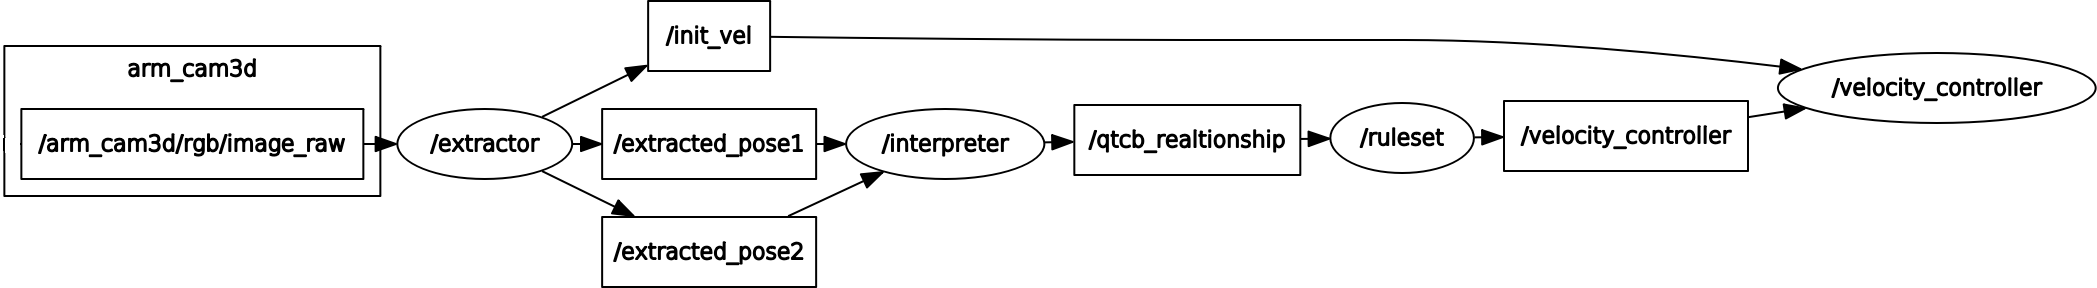
\includegraphics[scale=0.4]{images/rosgraph}
	\caption{A rosgraph image showing the pipeline for the developed approach, the rectangles represent the topics and the ovals represent the nodes.}
	\label{fig:rosgraph}
\end{figure}


\subsection{QSRLib}

\paragraph{Input Data Structure}To utilize the full capability of the QSRlib \cite{qsrlib}, we need to convert any raw data into the standard input format(`World\_Trace' object instance) that is accepted by this library. This `World\_Trace' \cite{qsrlib} contains various inbuilt methods that are used to convert the raw data into this format. The primary component of `World\_Trace' is a python dictionary called `trace', this dictionary uses the timestamps as its keys while the object instances of the `World\_Trace' class represent the values in this dictionary. Any `World\_State' object instance encodes the spatial objects as its primary member, this object instance is structured as a dictionary. The keys of this dictionary are represented by unique names of the spatial objects while the values are represented as object instances of the `Object\_State' \cite{qsrlib} class. An object instance of the 'Object\_State' contains data regarding spatial objects at any particular instance of time.

\paragraph{Output Data Structure}Like the standard format for input data, the output of the QSRLib also follows a standard output structure, this data structure is an object instance of the type `World\_QSR\_Trace' \cite{qsrlib}. Similar to the input data structure the primary element of this data structure is also `trace', implemented in the form of a dictionary whose keys are the timestamps of the QSRs. These keys match the timestamps of the object instance of `World\_Trace'. The values of this dictionary are the object instances the `World\_QSR\_State' class. The `World\_QSR\_State' object instance uses the `qsrs' as its primary element, such that the `qsrs' is a dictionary which encodes unique combinations of the spatial objects as its keys and object instances of the QSR class as its values.
\subsection{Perception}
\paragraph{} The perception module is built into a single ROS node using the python 3 language and utilizes various libraries to process the video data received from the camera. The video data is published on the `arm\_cam3d/rgb/image\_raw' topic in the ROS image format, to utilize this data for detection of the markers we convert it into OpenCV images format using the inbuilt ROS `cv\_bridge' package. To generate and detect the markers we use an inbuilt dictionary from the OpenCV aruco module (`cv2.aruco'), which contains 250 different markers each of the size `6X6'(36 bits). Once the raw data is converted into an OpeCV image format, we can run the `aruco.detectMarkers()' method to detect markers and extract their respective marker\_id, along with their pose(using `aruco.estimatePoseSingleMarkers()' method) and the time of their detection. Once a marker is detected its pose in the real world is estimated with the help of the camera matrix (allows the us to map 3d points to the 2D image and vice-versa). The units used for the pose of the markers depends upon the units used to depict the length of one side of the marker, as we have specified this in meters the final pose of the markers is also in meters.

\paragraph{} Since we use atleast two markers at corresponding positions on the opposite walls we needed a method to ensure that all the data from both the markers is published at all times and that there is no mix-up of the data, hence to achieve this we make use of two separate publishers for both the markers and to ensure that there is no mix-up we bind each publisher to a single `marker\_id' by using a clever combination of flag variables and if-else conditions. To enable cross checking the marker's ID number is stored until the robot has moved past that particular set of markers. Since we use two publishers we also use two individual topics(`extracted\_pose1' and `extracted\_pose2') to which these publishers publish their respective marker information. Finally custom messages are used to publish the data to the topics, this message encodes the the time-stamp of the marker detection, the marker id number and a 3D pose vector that contains the Cartesian coordinates for each marker.

\subsection{Representation}
\paragraph{} Like the perception module the representation module is also implemented using ROS and python 3 within a single node, while we use two different nodes for the two calculi the base approach for both remains the same(as discussed earlier).

\paragraph{QTCB Implementation :} The marker data published to the topics `extracted\_pose1' and `extracted\_pose2' serves as the raw data for this node. The data is filtered using the `ApproximateTimeSynchronizer()' method from the ROS `message\_filters' module, this filtering ensures that only marker data that is atmost 0.1 seconds apart will be used for further processing. Upon filtering the data we obtain the marker information for atleast two markers that have been detected at similar instants of time thus ensuring that we always deal with the most recent data. Furthermore the pose vector of both these markers is analyzed to decide which marker lies to the left and which one lies to the right, this is done by checking the values of their X-coordinates(if negative it lies on the left otherwise right) the respective marker ids are then stored as part of the custom message(QsrMsg) that will be published on the `qtcb\_realtionship' topic from where it is picked up by the control module and used as a reference during the decision making process. Since we are using the QSRLib to obtain the $QTC_B$ relations we need to first convert the raw data into the format utilized by the library. To do so we utilize the `World\_Trace' data structure provided by the library, which incidentally also happens to be the primary form to which the raw data needs to be converted. 

\paragraph{}To begin with we create the `Object\_State' tuple that contains the Cartesian coordinates of the markers, the distinct object name for the marker, a common time stamp for when the marker was detected. For the $QTC_B$ calculus we need atleast two instances of each individual object at consecutive instances of time, as the $QTC_B$ checks the variation in the object's position to determine if the object has moved(further inference is then used to qualitatively represent the objects motion) or not. The next step is to wrap the defined `Object\_State's' in a list and store them in unique variables to add them as individual entities to the `World\_Trace' data structure. The Cartesian coordinates for all the objects and the robot are initialized as (0,0) and get updated when new data is available to the node, for the sake of simplicity the Cartesian coordinates of the robot are always fixed at (0,0) this does not affect the overall functionality of the algorithm in any way and can be physically interpreted as egocentric motion of the robot with respect to its environment. Finally after defining this time-series of the object's states we can finally add this data to the object of type `World\_Trace' using the inbuilt `add\_object\_state\_series()' method (this takes as argument the object list of time-series data that was defined earlier). After adding all the `Object\_States' to the `World\_Trace' object instance we can finally wrap it up in the form of a `QSRlib\_Request\_Message' which includes the converted data in the from of a `World\_Trace' object instance along with desired calculi (selected from a list of available calculi in the QSRLib) and any runtime arguments that are specific to the calculi in  consideration. These runtime arguments are called as `dynamic\_args' and are unique for each calculi. In the case of our implementation of the $QTC_B$ these `dynamic\_args' are the `no\_collapse',`quantisation\_factor', the no collapse tells the library to avoid collapsing the output amongst timestamps if there is no change in the relative movement/trajectory of the objects, whereas the `quantisation\_factor' represents the minimum change in position that should be considered to assume that the object has moved(0.01 meters in our case). The completed `QSRlib\_Request\_Message' is then sent to the `qsrlib\_ros\_server' to obtain the qualitative representation of the relative trajectories of the objects.

\paragraph{} Since the relations obtained from the `qsrlib\_ros\_server' are mutually exhaustive the relations, complimentary repeated relations exist for the given set of spatial objects this excessive data is often unnecessary, therefor we also specify beforehand the specific set of spatial objects for which we want the qualitative relations, using the `dynamic\_args'. The response obtained from the `qsrlib\_ros\_server' is sorted according to the timestamps and looped through using to obtain the objects in the relationships and the respective relations themselves. Once this is done the data is put into a custom message that contains the message time, the marker id's, the id's of the left and right markers, the objects in a relationship and the relationship itself. After filling up the message with all this data it is published to the `qtcb\_relationship' from where it can be picked up by the next node and utilized for making motion updates to the robot's movement.

\paragraph{ARGD Implementation :} The implementation of the $ARGD$ calculus is the similar to the one described above for  $QTC_B$ calculus, with the only difference occurring in specific `dynamic\_args' used for this calculi. Specifically these are `qsr\_relations\_and\_values' which define the distance thresholds and the corresponding relationship for these thresholds, for our use case we define the thresholds as follows `{`Near': 3.0, `Medium': 3.5 , `Far': 4.0}' in the form of an immutable dictionary. All the values specified for the thresholds are in meters and relate to each other using the `less than($<$)' relational operator(unlike what is mentioned in \cite{gatsoulis2016qsrlib}), hence any distance value below three meters is considered as `Near' while any distance value above four meters is considered `Far', for values that lie between any of the defined threshold the assigned relation is always that of the lower threshold, for instance if the distance value is `3.7' meters then the corresponding relation will be `Medium'.

\paragraph{}Another difference from the $QTC_B$ implementation is that for the $ARGD$ we use only a single instance of the `Object\_State' tuple for each individual object, this is because unlike the $QTC_B$ calculus which uses distance as a means to approximate the objects trajectory, the $ARGD$ uses the distance as the absolute measure of the objects position with respect to other spatial entities, no trajectory or path information is abstracted from the distance data. The reason for this lies in the definition of the distance calculus which states that this calculi is used to qualitatively abstract distances between static objects, hence eliminating the need for any sort of temporally augmented trajectory data. As mentioned in the previous section(QTCB Implementation), the data from this node is published using the custom message `QsrMsg' to the `argd\_relationship' topic. The composition of this message varies slightly from the one presented in the `QTCB Implementation', while the `QsrMsg' for the $QTC_B$ contains the relations between the robot and any one marker at any given instance of time the `QsrMsg' for the $ARGD$ contains the relations between the robot and any both the markers at any given instance of time. The reasons for this will be explained further in the next section of this chapter.

\subsection{Control}
\paragraph{}The control module also uses two different nodes to deal individually with the $QTC_B$ and $ARGD$ relations, this structure promotes modularity and makes it easier to combine the two pipelines if the need ever arises. Furthermore the control module is divided into two ROS nodes one for interpreting the relations and the other for converting these motion updates into numerical velocity values that can be used to control the robot.

\paragraph{QTCB Controller}
\paragraph{}The control module is implemented as a set of if-else rules that compare the relations obtained from the representation module and present a possible control command that is to be applied to the robot's motion. After obtaining the relations on the `qtcb\_relationship' topic the data is preprocessed using python string operators such as split() and strip() to obtain the individual sets of objects(eg:(object1,robot)) and their corresponding relationships again the relationships are checked to verify that they do actually belong to the $QTC_B$ calculi, since each relationship has this encoded in the form of the calculi name a simple string check suffices for this purpose. Once the relations have been cleaned we use simple if-else conditions to check for possible matches from a set of possible relations, this is feasible as there exists a finite set of relations that are can exist between the two objects, also since the relations between the robot and the two markers are mutually exhaustive it suffices to check the relation of each marker with the robot individually as we know that the corresponding relationship with the other marker is the inverse of the relationship between the current marker and the robot. Furthermore this trick allows us to compare the relationships amongst each set of objects individually and reduces the number of possible states that have to be compared, for a relation between two individual objects there are 9 possible relationships, hence there are 9 possible relations for each object set, now if we decide to combine two object sets then we have a set of 81($9^2$) possible relationships for only one order of combination of these object sets, if the order is now reversed then we get another set of 81 possible relationships, hence to make this a set of mutually exhaustive relations(for only two object sets) we have to go through a set of 162($2 X 81$) possible relations to obtain one possible update for the robot's motion thus making this an unnecessary complication that can be avoided. Also this number rises exponentially if the number of objects or markers is increased as the object sets are possible combinations of these individual markers this adds an unnecessary dependency on the number of markers. Therefore to avoid such complications we compare the relations for each object set individually and use the simple information of the relative location(left or right) of the object with respect to the robot to decide upon the motion update for the robot. Thus resulting in a simple yet effective control module. Additionally $\{-,+,0\} = [towards, away, stable]$, are the actual interpretations of the $QTC_B$ relations when the robot has allocentric spatial transforms with respect to the environment, but in our case since the robot is considered to have egocentric spatial transforms with the environment the relations are inverted. 

\paragraph{ARGD Controller}
\paragraph{} Similar to the `QTCB Controller' the control module for the $ARGD$ also uses if-else rule-sets to iterate through a list of possible relations and then select a motion update when a match is found, unlike the $QTC_B$ though we do not compare the relations of each object set individually as the number of relations for each object set is very small(3) and here the combinations of the object sets is necessary to be able to distinguish between different states of the robot with respect to the objects or markers, again the implementation of this rule-set ensures that it is independent of the number of markers and their placements in the environment(as can be seen from the experiments).
\paragraph{}Since in this case we use a combination of the relations of the object sets, the data obtained from the `argd\_relationship' topic is processed slightly differently from the manner shown in the `QTCB Controller' section. Here we apply the python string operators `split()' and `strip()' to breakdown the breakdown the raw relationship data into parts so that it is easy to associate them with their respective object sets. Once this is done we use the if-else conditions to iterate over the various possible combinations of these individual relations to obtain a suitable motion update. 

\section{Implementation Notes}
\begin{itemize}
	\item The current implementation assumes that there are at least two markers in the environment at any given point of time. This is the core assumption around which the entire implementation is built.
	
	\item The approach is heavily dependent on the perception module, the robot moves according to what it sees. If we want to remove the dependency on the use of markers then we need a robust perception module that can track features such as notice boards etc. this may be achieved by using computer vision techniques such as template matching or optical flow analysis.
	
	\item Currently the controllers used in the approach are configured to move the robot forward through the corridor and cannot deal with corner's and dead ends, to allow the robot to deal with such situation additional controller nodes can be implemented that allow such behaviors to be executed safely. In such cases only the controller node needs to be changed in a manner that provides a new rule-sets for these particular situations. 
	
	\item Additionally we assume that a minimum of two objects(discounting the robot) are necessary for the robot to build valid relations and successfully navigate through the corridor environment, thus forcing the relationships to be built for only three object sets ([object1, robot], [object2, robot] and [object1, object2]) and enforce this using the `dynamic\_args' argument for the QSRLib.
\end{itemize}